\documentclass{article}
% \usepackage[portuges]{babel}
% \usepackage[utf8]{inputenc}
% \usepackage[T1]{fontenc}
\usepackage{hyperref}
\usepackage{url}
\usepackage{graphicx}
\usepackage{float}
\usepackage{enumerate}
\usepackage{makeidx}
\usepackage{booktabs}
\usepackage{pdfpages}
\usepackage{a4wide}

\setlength\oddsidemargin{0.3in}
\setlength\evensidemargin{-0.3in}
\setlength\headsep{15pt}
\setlength\footskip{30pt}

\usepackage{fontspec}
\defaultfontfeatures{Mapping=tex-text}
\setmainfont[
  Extension=.ttf,
  Path=font/,
  Scale=1.00,
  BoldFont={NewsGotTMed Regular},
  ItalicFont={NewsGoth Lt BT Light},
  ItalicFeatures={FakeSlant},
  AutoFakeSlant=0.3,
  BoldItalicFeatures=FakeSlant, 
]{NewsGotT Regular Fixed}

%Line Spacing
\usepackage{xspace}
\usepackage{setspace}
\onehalfspacing

% Language definitions
\usepackage{polyglossia}
\setmainlanguage{portuges}


% environment created for organization purposes, only.
\newenvironment{TODO}{%
  \color{blue} \itshape \begin{itemize}
}{%
  \end{itemize}
}

%---------------------------------------

% our addimage command
\newcommand{\addimg}[1]{%
  \begin{center}
    \includegraphics[width=0.75\textwidth]{#1}
  \end{center}
}

\newcommand{\RowStretch}[1]{\renewcommand{\arraystretch}{#1}}



%----------------------------------------------------------

\begin{document}

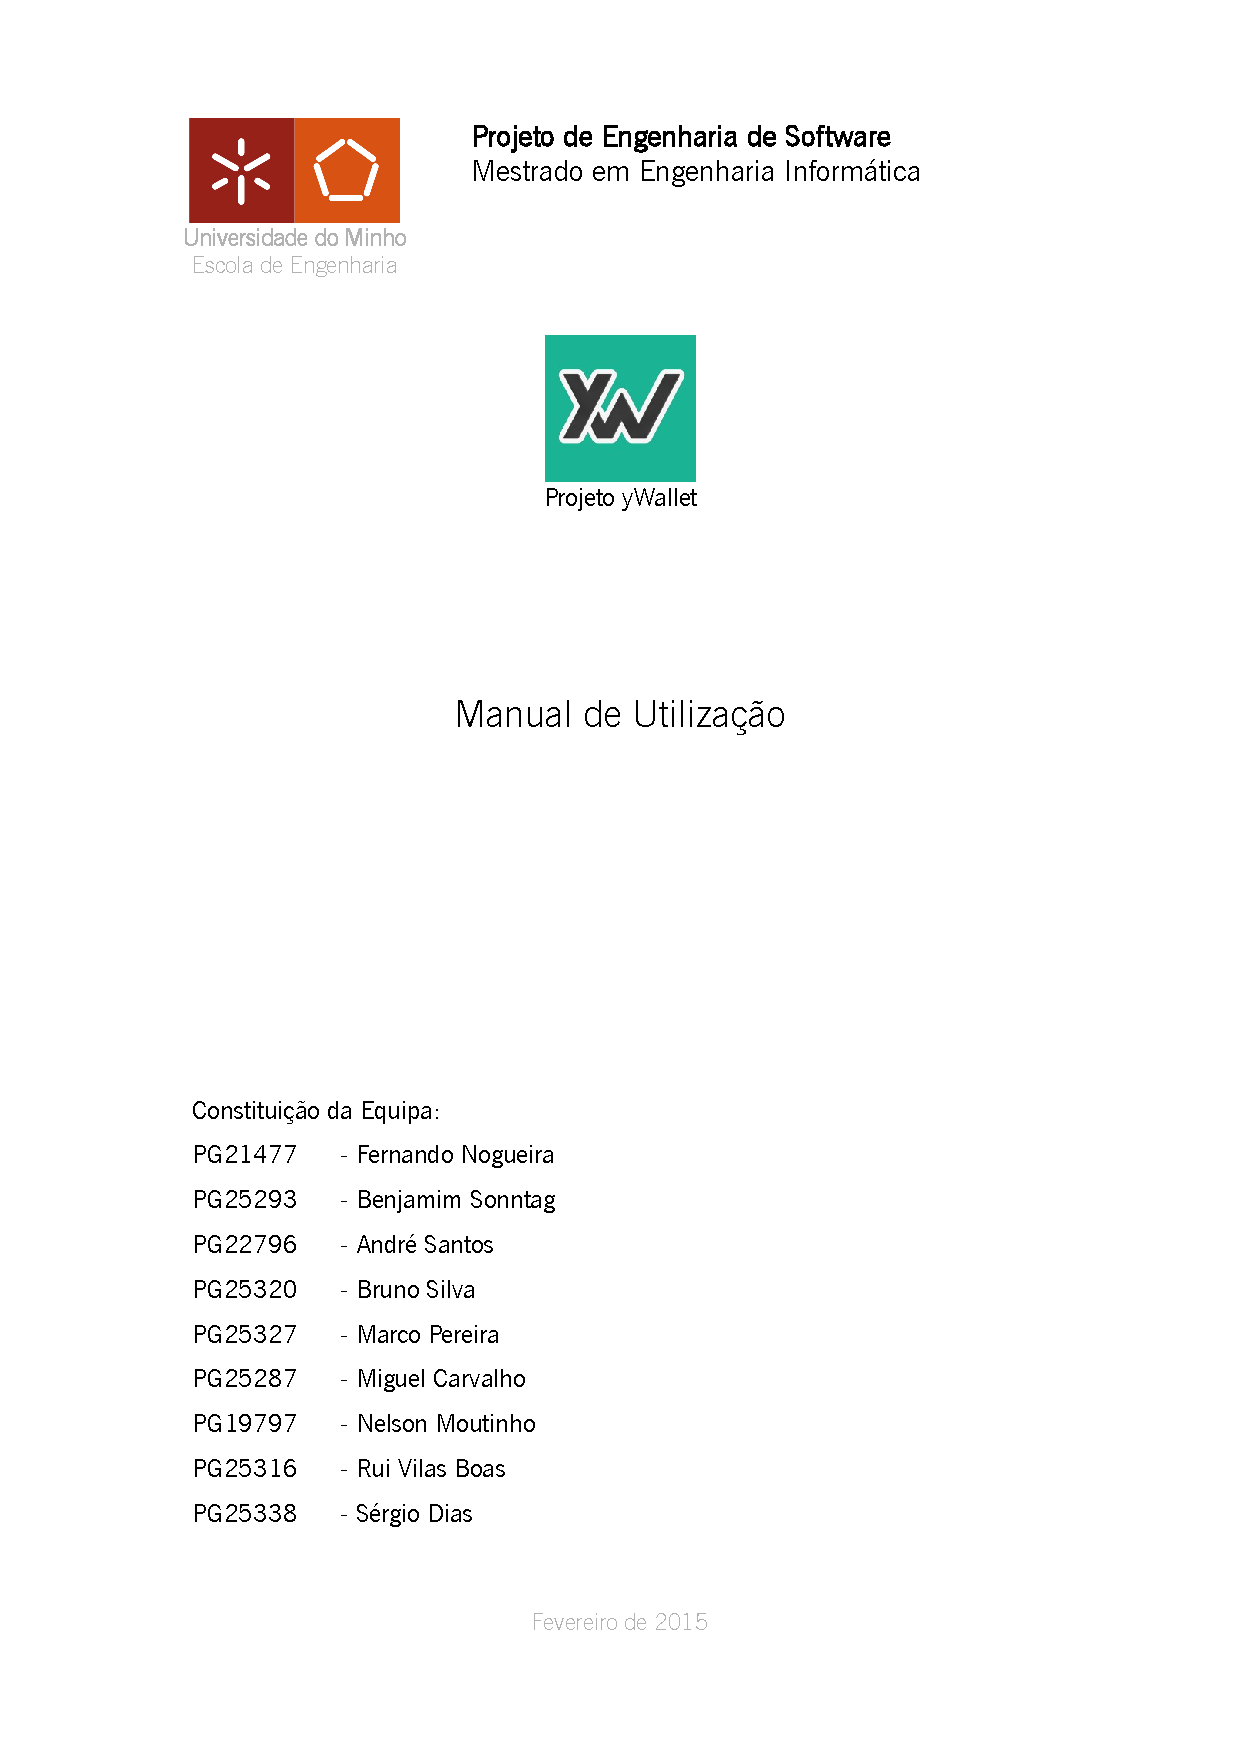
\includepdf[pages=-]{capa}

\tableofcontents

\pagebreak

  \section{Introdução}
  O presente documento tem como objetivo explicar como se utiliza a aplicação \textit{yWallet}. Após a leitura do documento é possível o utilizador começar a utilizar a aplicação. A \textit{app yWallet} foi construída com o objetivo de ser simples e intuitiva por forma a que os utilizadores a consigam utilizar sem recorrer à leitura deste documento. 

  O documento está organizado em várias secções, que correspondem às funcionalidades da aplicação, onde se descreve e ilustra os ecrãs da respetiva funcionalidade.

  Qualquer dúvida pode ser esclarecida através do \textit{website} da \textit{yWallet}: http://ywallet.co (ver Figura \ref{website}). Está disponível a api utilizada pela aplicação da yWallet em http://ywallet.co/api (ver Figura \ref{api})

  \begin{figure}[H]
    \begin{center}
      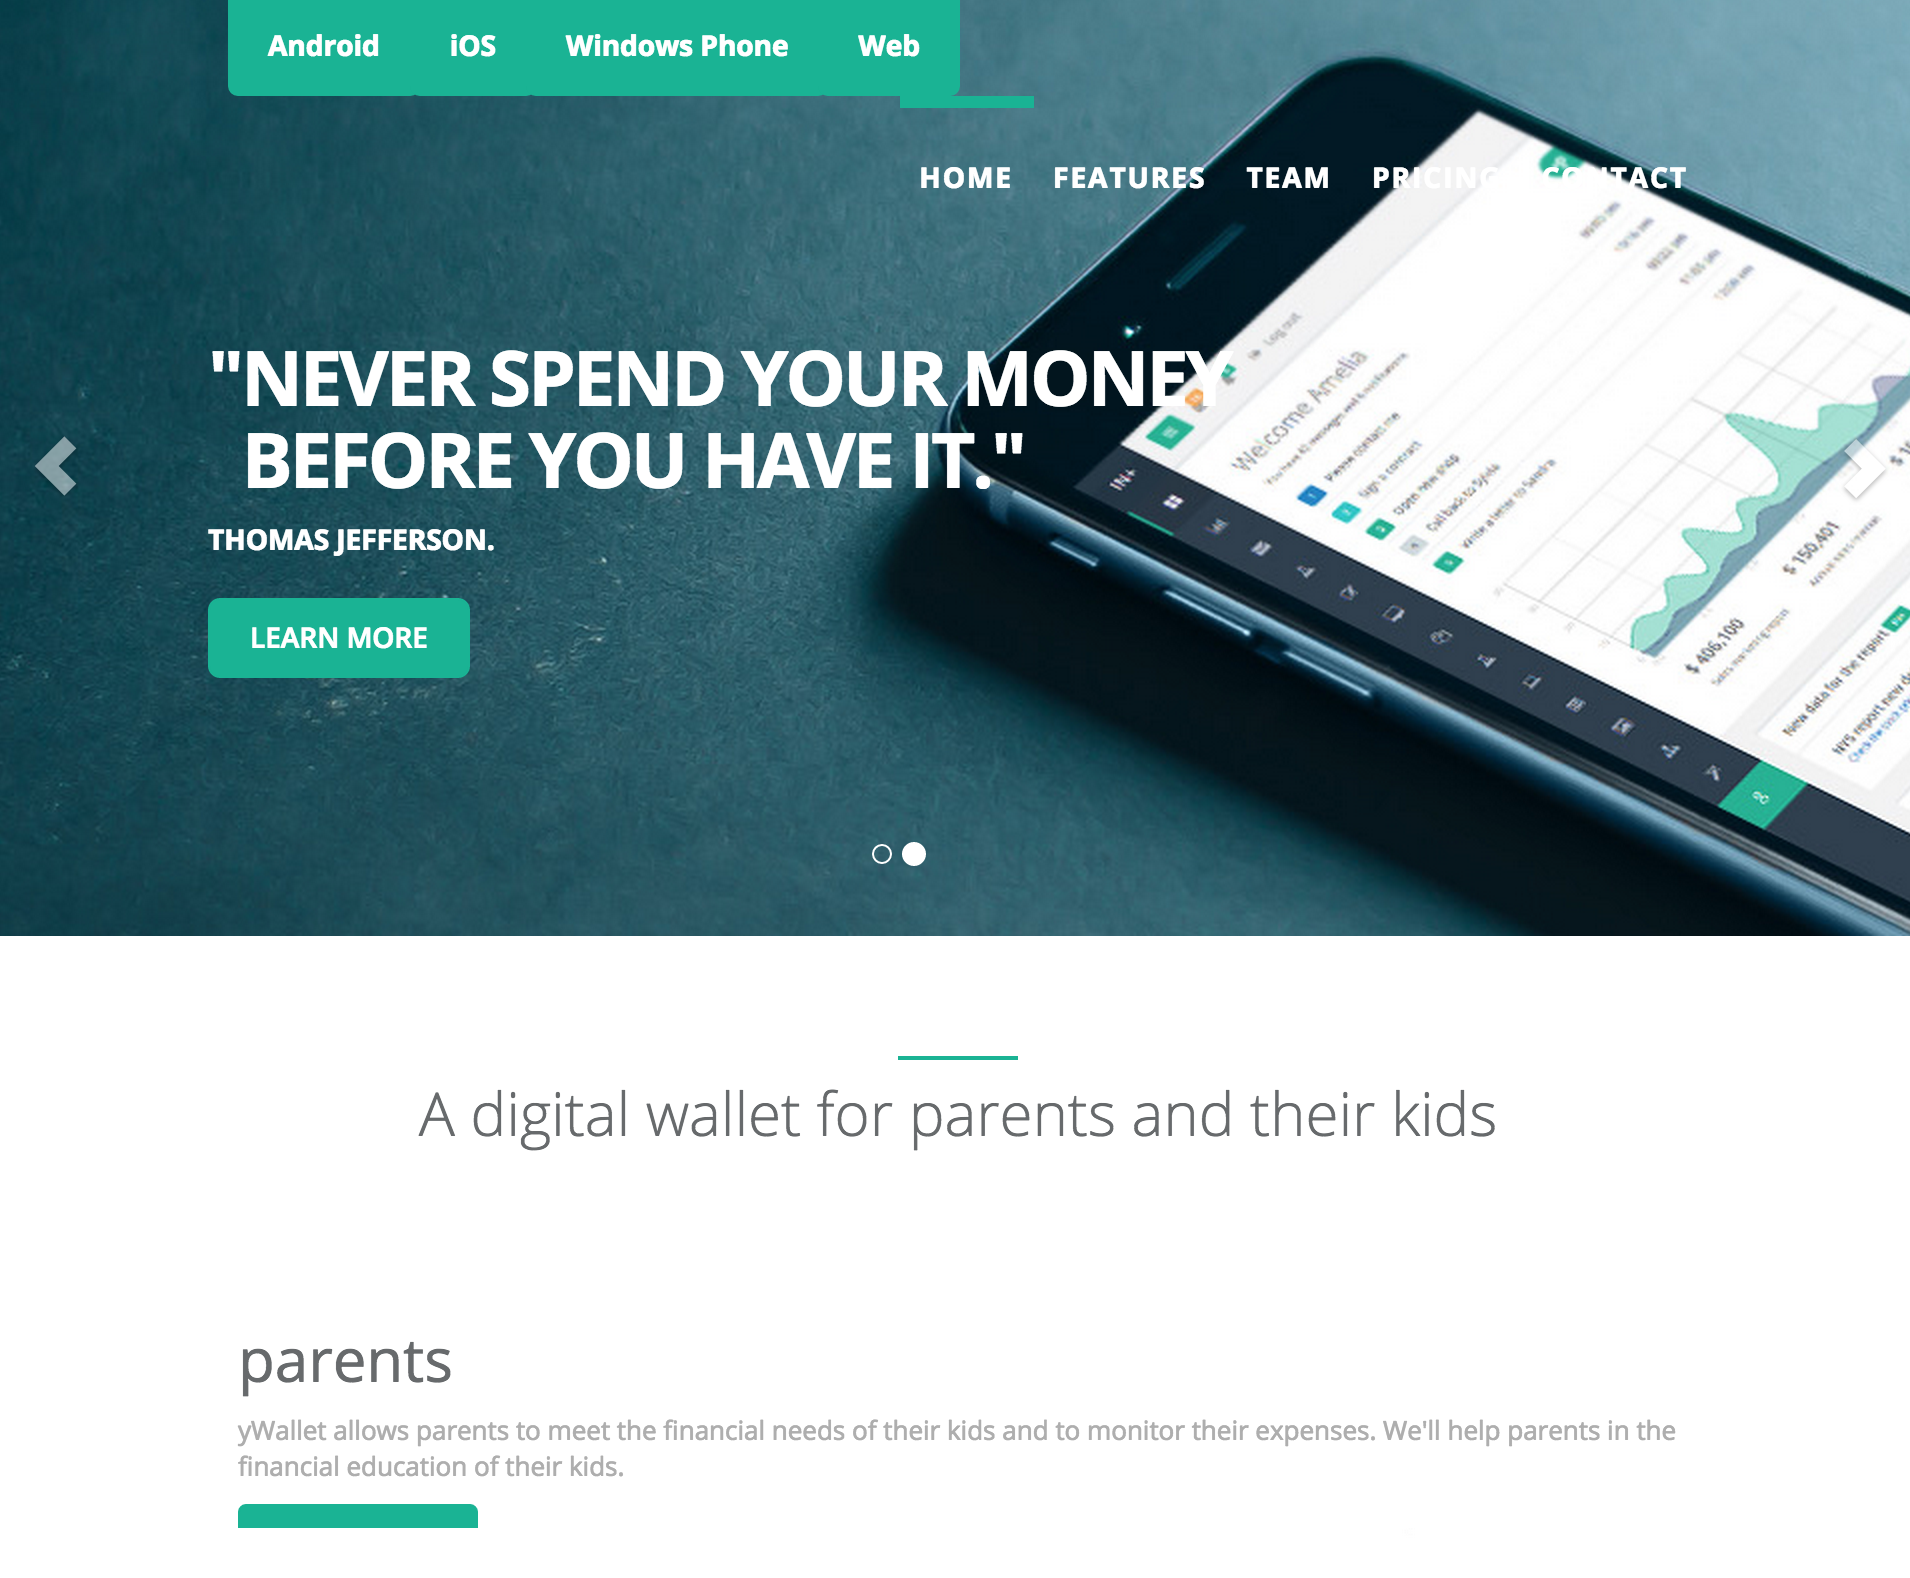
\includegraphics[width=0.5
      \textwidth]{website.png}
    \end{center}
    \caption{\textit{Website yWallet}}
    \label{website}
  \end{figure}

  \begin{figure}[H]
    \begin{center}
      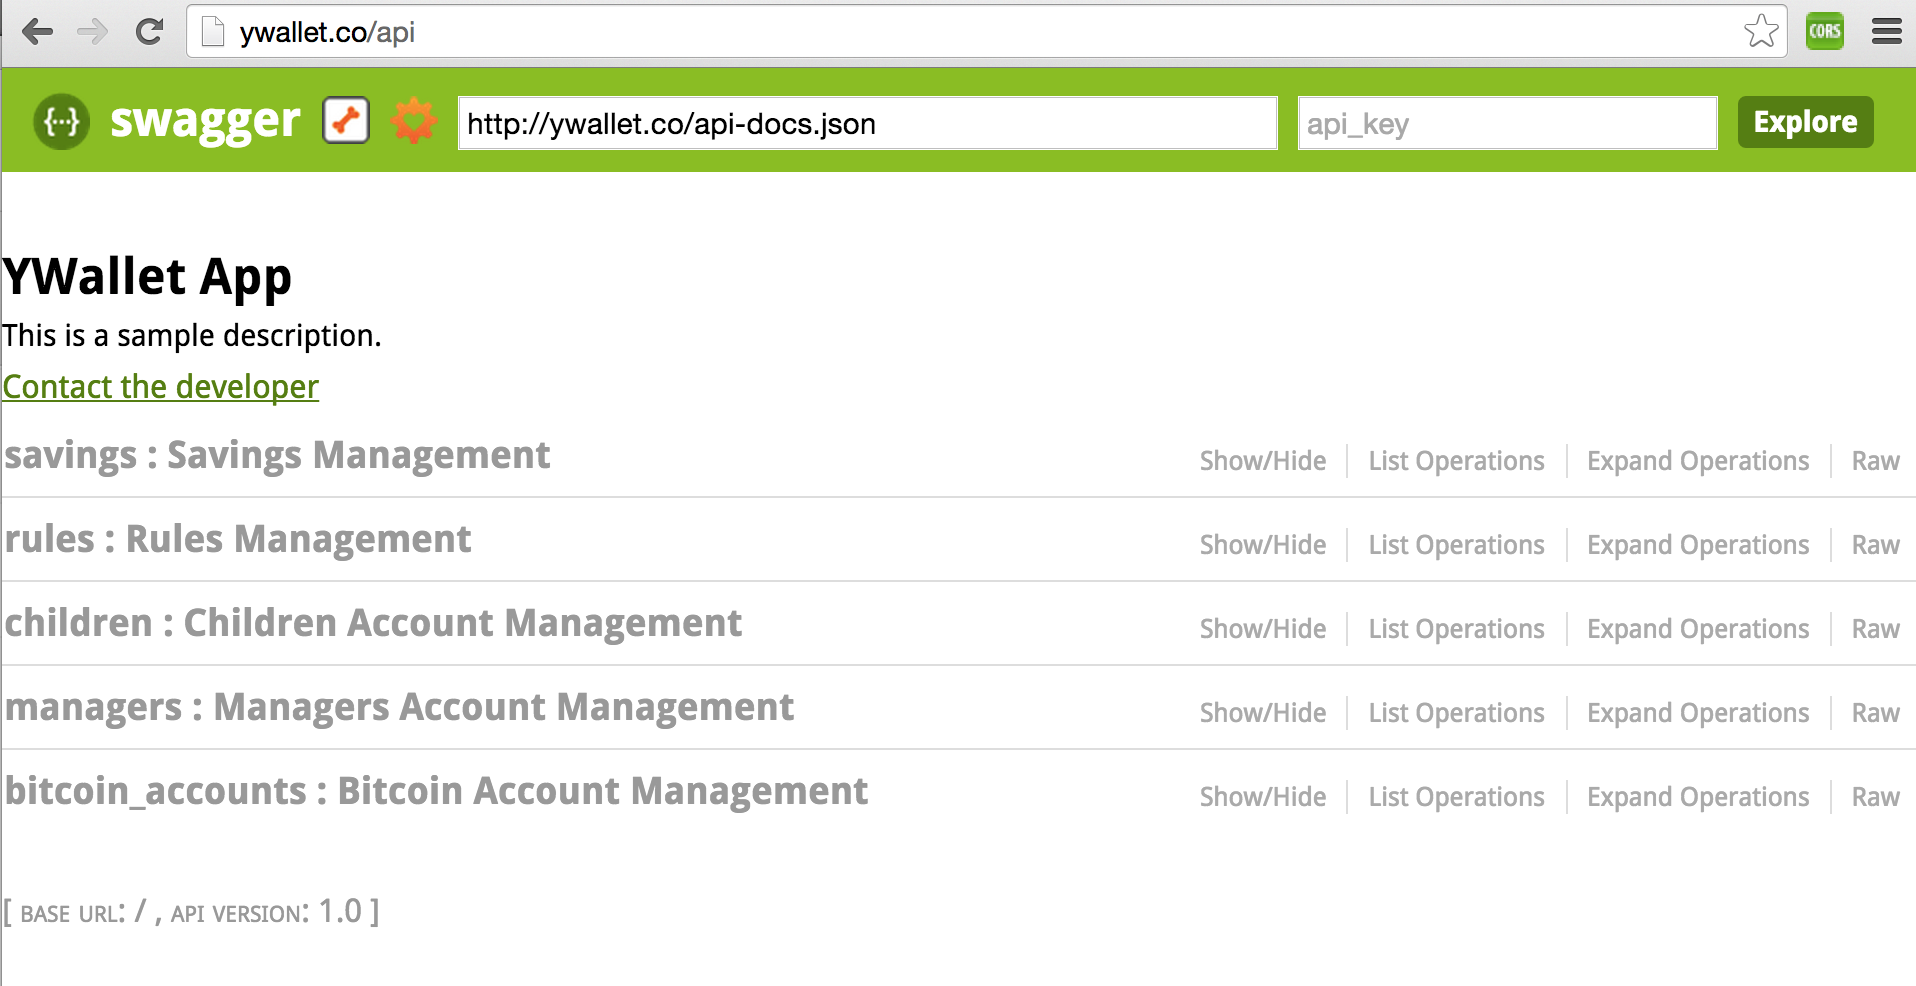
\includegraphics[width=0.5
      \textwidth]{api.png}
    \end{center}
    \caption{\textit{API yWallet}}
    \label{api}
  \end{figure}

  \pagebreak

  \section{Autenticação}  
  \begin{figure}[H]
  \begin{center}
    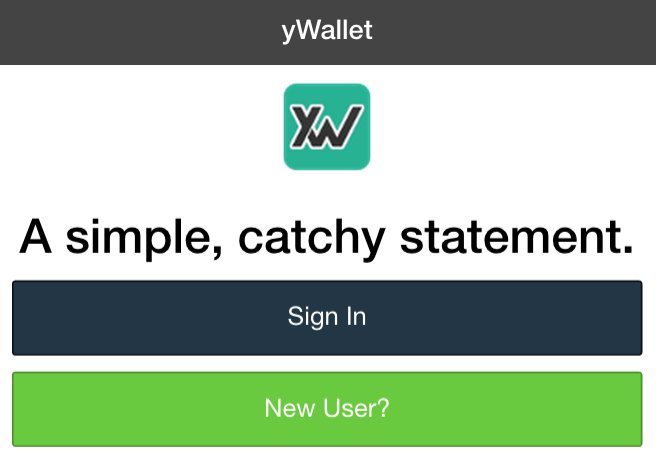
\includegraphics[width=0.5
    \textwidth]{authentication/init.png}
  \end{center}
  \caption{Autenticação}
  \label{fig:1}
\end{figure}

No ecrã de autenticação, é apresentada ao utilizador a possibilidade de registo e de \textit{login} na aplicação.

\subsection{Registo}
  \begin{figure}[H]
    \begin{center}
      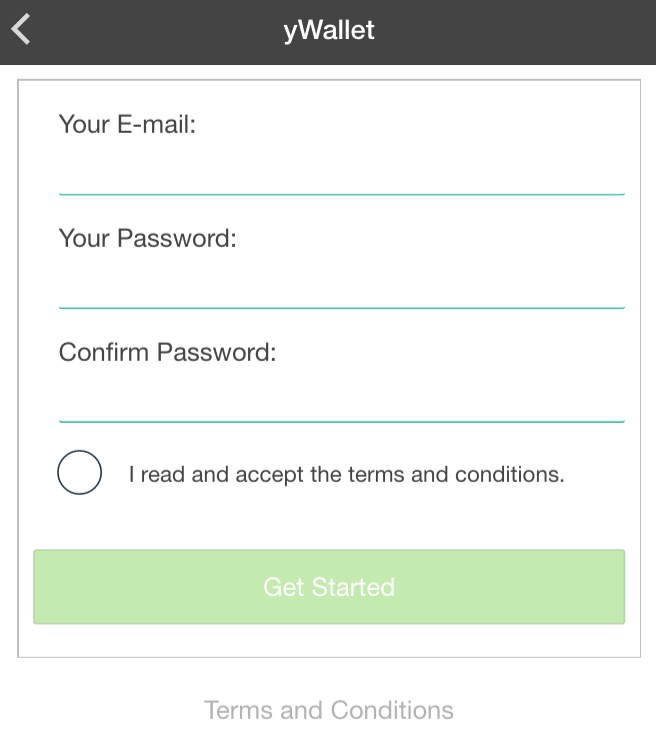
\includegraphics[width=0.5
      \textwidth]{authentication/register.png}
    \end{center}
    \caption{Registo}
    \label{fig:1_1}
  \end{figure}

Para utilizar a aplicação é necessário o utilizador já ter uma conta  \textit{Coinbase}. Caso não tenha existe a possibilidade de criar no processo de registo. Para criar o registo apenas é necessário o email do utilizador e uma \textit{password}. Apenas os pais (\textit{managers}) necessitam de criar conta. Os filhos são adicionados pelos pais. (ver secção \ref{sec:conf}).

\subsection{Login}
  \begin{figure}[H]
    \begin{center}
      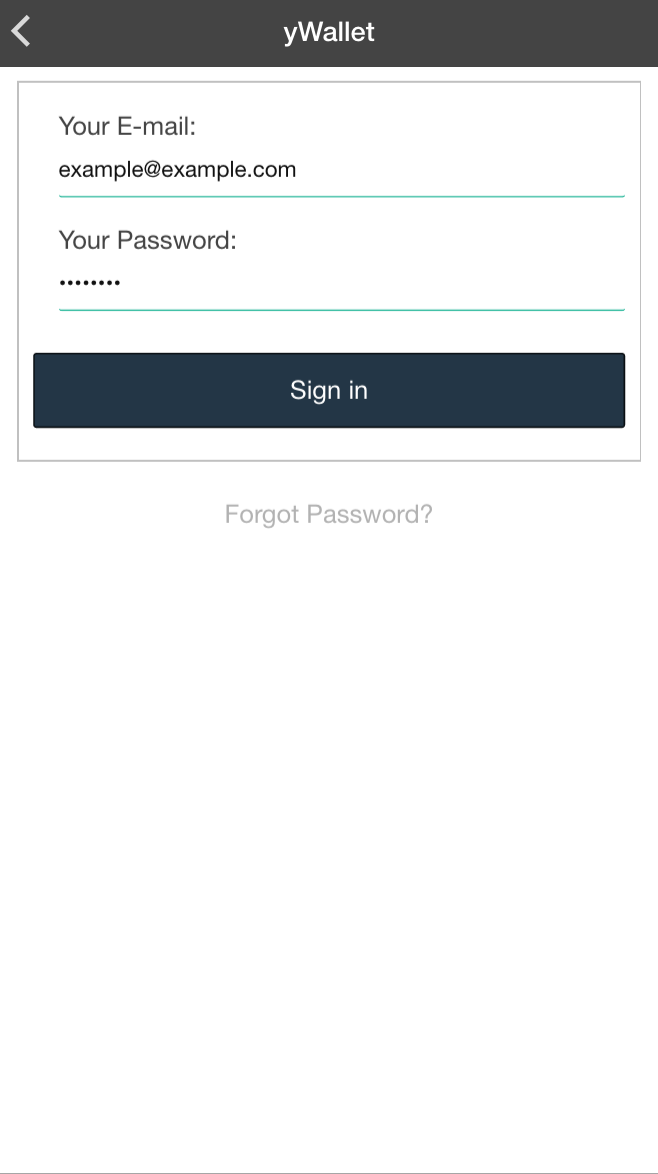
\includegraphics[width=0.5
      \textwidth]{authentication/login.png}
    \end{center}
    \caption{Login}
    \label{fig:1_2}
  \end{figure}

A Figura \ref{fig:1_2} apresenta o ecrã de \textit{login} na aplicação.

\subsection{Recuperar a \textit{Password}}
  \begin{figure}[H]
    \begin{center}
      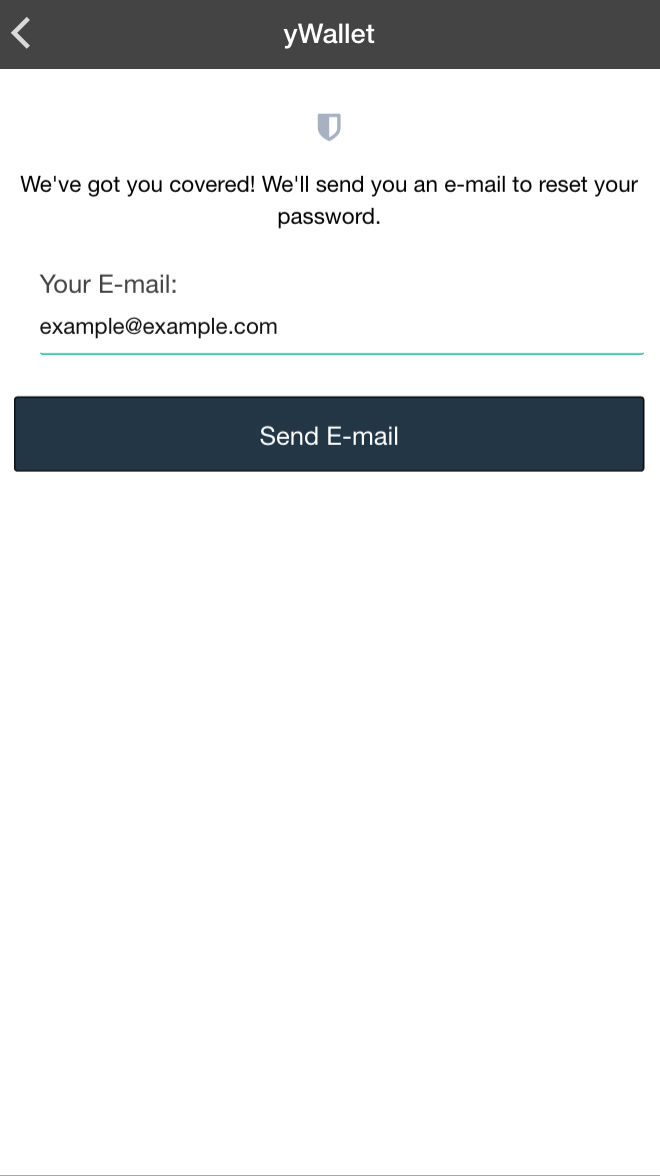
\includegraphics[width=0.5
      \textwidth]{authentication/forget.png}
    \end{center}
    \caption{Recuperar Password}
    \label{fig:1_3}
  \end{figure}

Caso o utilizador não se lembre da \textit{password} é possível recuperar utilizando a opção \textit{Forgot Password?} do ecrã de \textit{login} (Figura \ref{fig:1_2}). O ecrã de recuperação da \textit{password} é apresentado na Figura \ref{fig:1_3}.

  \section{Menu}  
  \begin{figure}[H]
	\begin{center}
		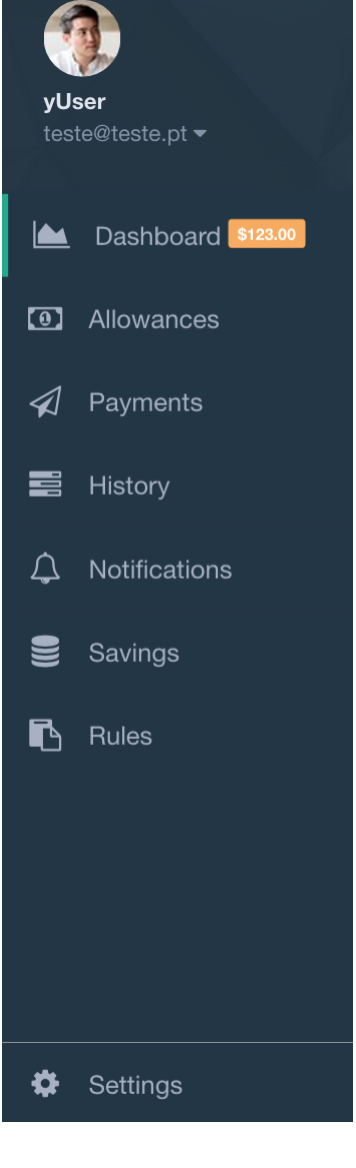
\includegraphics[width=0.25
		\textwidth]{menu/menu.png}
	\end{center}
	\caption{Menu da aplicação}
	\label{fig:10_1}
\end{figure}

O menu lateral possibilita a navegação pelos vários ecrãs da aplicação. Os ecrãs mostram a informação de acordo com o utilizador ativo que pode ser selecionado no menu. Para os pais com vários filhos verem a informação de cada filho basta selecionar o filho como utilizador ativo. 

  \section{\textit{Dashboard}}
  \begin{figure}[H]
	\begin{center}
		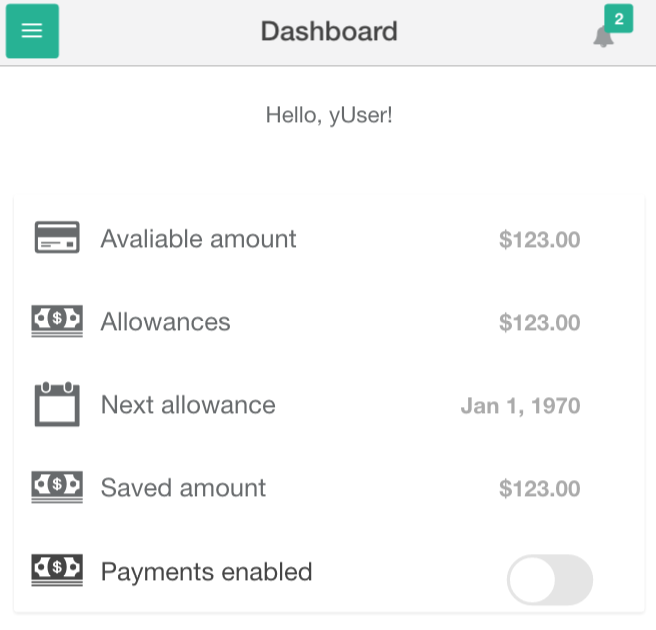
\includegraphics[width=0.5
		\textwidth]{dashboard/dashboard.png}
	\end{center}
	\caption{Dashboard}
	\label{fig:2}
\end{figure}

A \textit{Dashboard} apresenta o estado da conta do utilizador ativo. Os pais podem ver a informação de cada filho, incluindo a informação da \textit{Dashboard}.

  \section{Mesadas}
  \begin{figure}[H]
	\begin{center}
		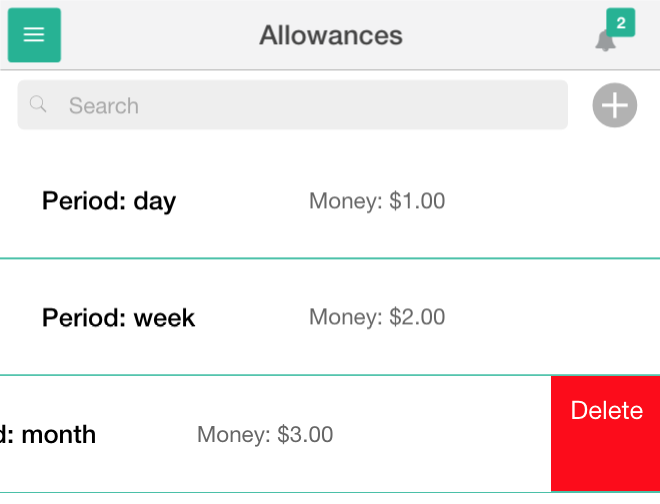
\includegraphics[width=0.5
		\textwidth]{allowances/allowances.png}
	\end{center}
	\caption{Mesadas do utilizador}
	\label{fig:3}
\end{figure}

\begin{figure}[H]
	\begin{center}
		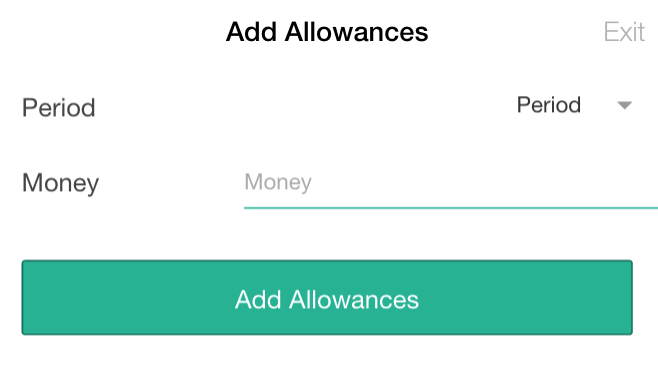
\includegraphics[width=0.5
		\textwidth]{allowances/addAllowances.png}
	\end{center}
	\caption{Adicionar Mesada}
	\label{fig:3_1}
\end{figure}

O ecrã que lista as mesadas (Figura \ref{fig:3}) apresenta as mesadas ativas. Para eliminar uma mesada é necessário arrastar a linha correspondente à mesada e selecionar o botão de apagar. Apenas os pais conseguem adicionar mesadas aos filhos. Para adicionar uma mesada seleciona-se o botão de adicionar no canto superior direito (Figura \ref{fig:3}). Será apresentado um novo ecrã onde é solicitado o período e o montante da mesada, por exemplo, vinte dólares por semana.

  \section{Pagamentos}
  \begin{figure}[H]
	\begin{center}
		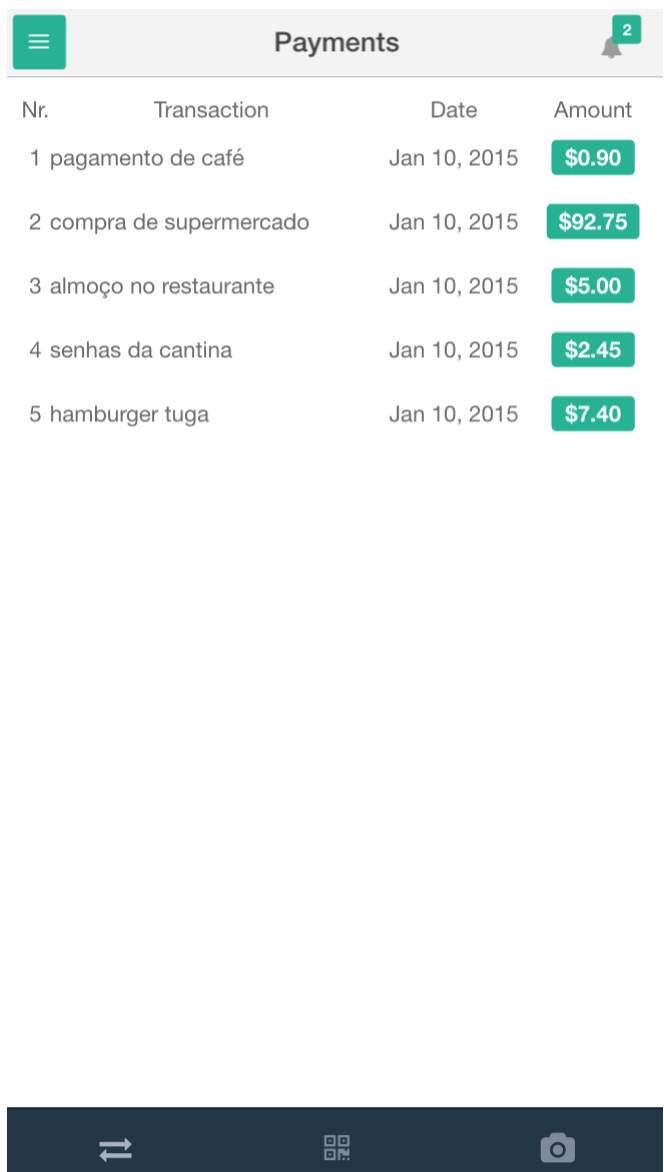
\includegraphics[width=0.5
		\textwidth]{payments/payments.png}
	\end{center}
	\caption{Pagamentos}
	\label{fig:4}
\end{figure}

\begin{figure}[H]
	\begin{center}
		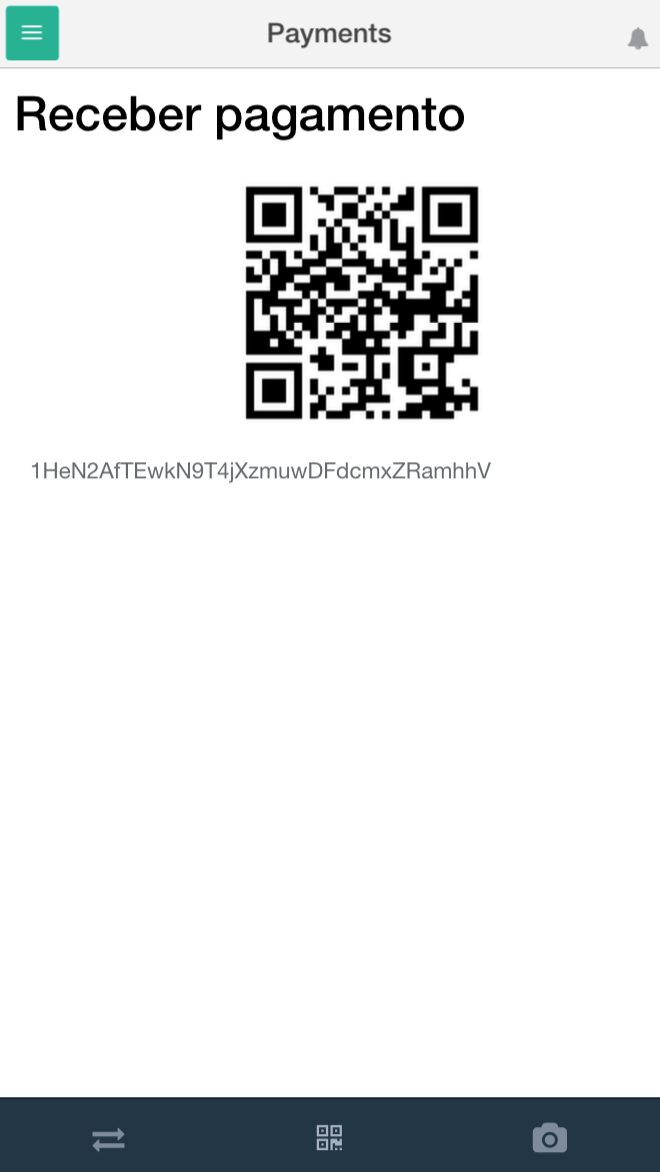
\includegraphics[width=0.5
		\textwidth]{payments/receive.png}
	\end{center}
	\caption{Receber Pagamento}
	\label{fig:4_1}
\end{figure}

O ecrã de pagamentos apresenta uma barra de navegação com três opções que se encontra no rodapé (ver Figura \ref{fig:4}). A primeira opção apresenta a lista de pagamentos, a segunda opção contém o \textit{QrCode} e o endereço \textit{bitcoin} para o utilizador receber dinheiro de outra pessoa (ver Figura \ref{fig:4_1}) e a terceira opção contém a opção de pagamento (ver Figura \ref{fig:4_2}).


\begin{figure}[H]
	\begin{center}
		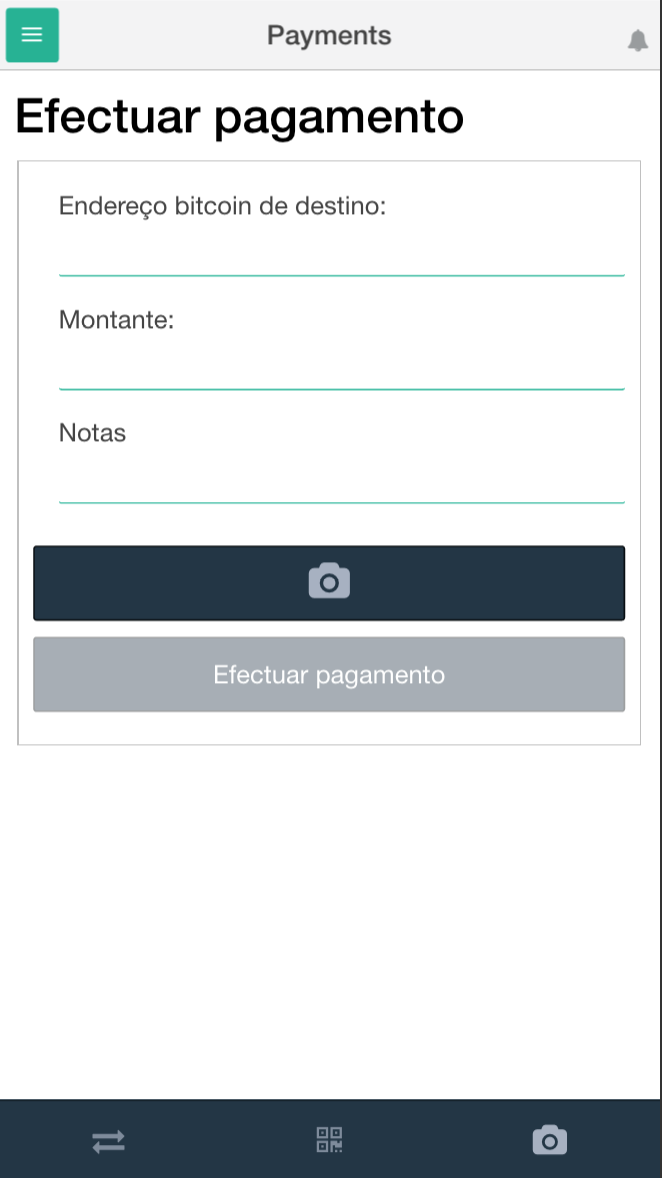
\includegraphics[width=0.5
		\textwidth]{payments/pay.png}
	\end{center}
	\caption{Pagar Despesa}
	\label{fig:4_2}
\end{figure}

 Na opção de pagamento é necessário inserir o endereço \textit{bitcoin} (ou usar o botão da câmara para obter o endereço através de um \textit{QrCode}), o montante a pagar e notas adicionais caso necessário.

  \section{Histórico}
  \begin{figure}[H]
	\begin{center}
		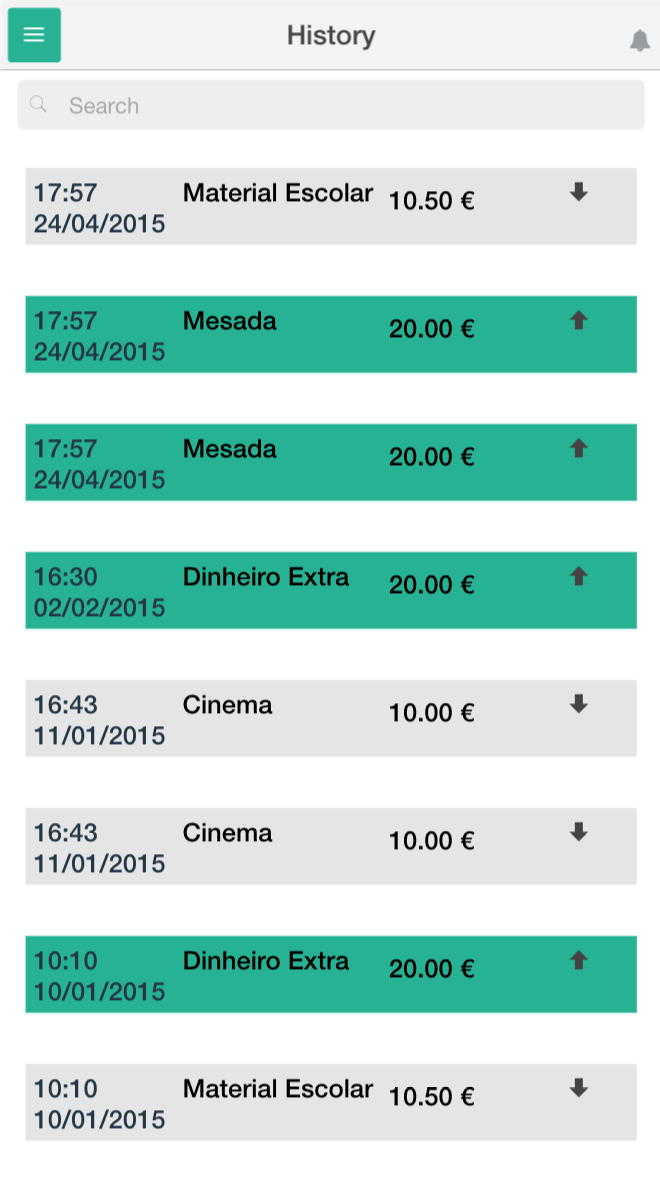
\includegraphics[width=0.5
		\textwidth]{history/history.png}
	\end{center}
	\caption{Listagem das transações}
	\label{fig:5}
\end{figure}

O histórico apresenta as transações (débitos e créditos) que o utilizador realizou com a aplicação.

  \section{Notificações}
  \begin{figure}[H]
	\begin{center}
		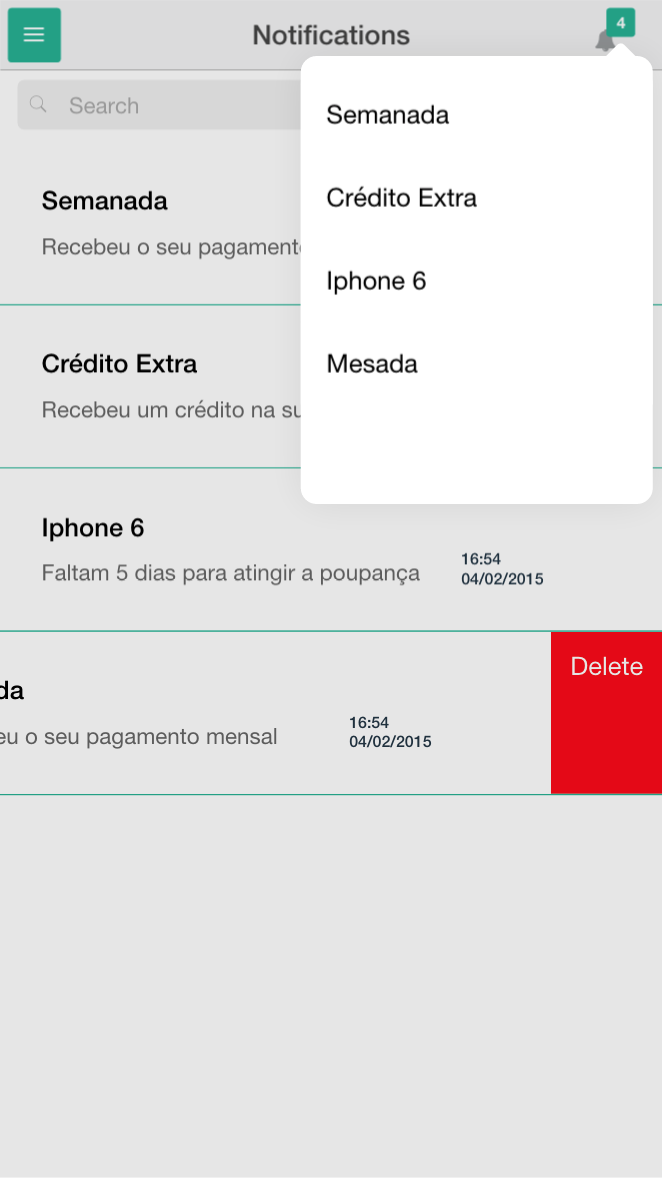
\includegraphics[width=0.5
		\textwidth]{notifications/notifications_widget.png}
	\end{center}
	\caption{\textit{Widget} de Notificações}
	\label{fig:6}
\end{figure}

É possível consultar as notificações mais recentes do utilizador selecionando o botão do canto superior direito presente em todos os ecrãs (ver Figura \ref{fig:6}).

\begin{figure}[H]
	\begin{center}
		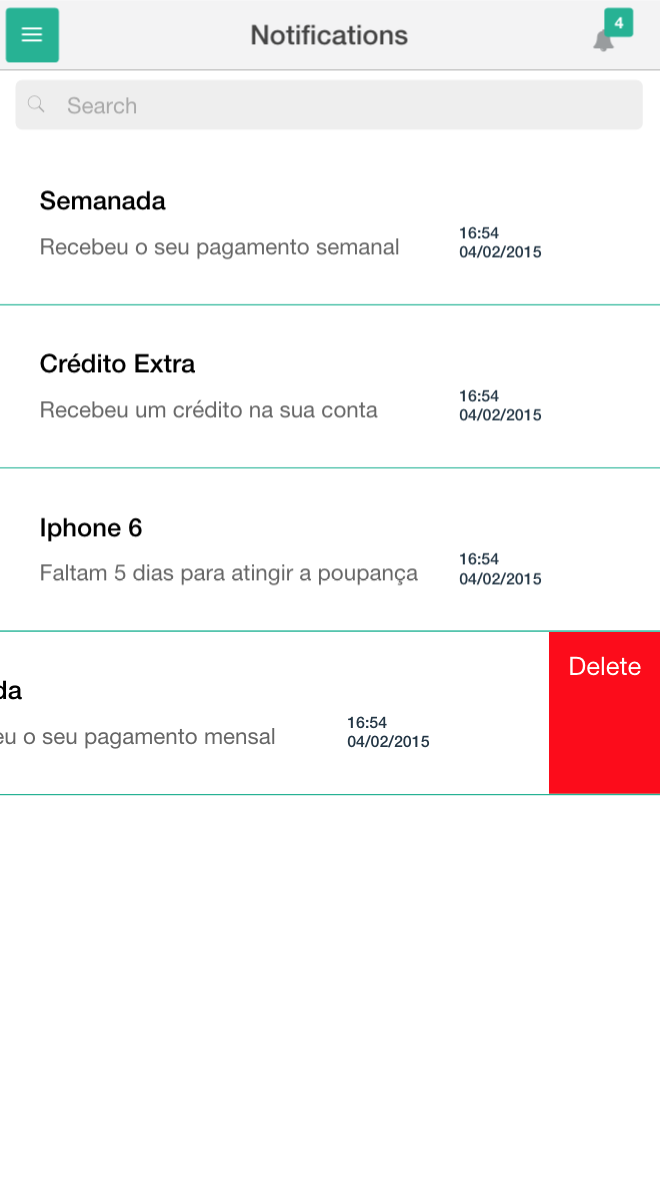
\includegraphics[width=0.5
		\textwidth]{notifications/notifications.png}
	\end{center}
	\caption{Detalhe das Notificações}
	\label{fig:6_1}
\end{figure}

É possível ver o detalhe e eliminar as notificações no ecrã de notificações acessível através do menu (ver Figura \ref{fig:6_1}).

  \section{Poupanças}
  \begin{figure}[H]
	\begin{center}
		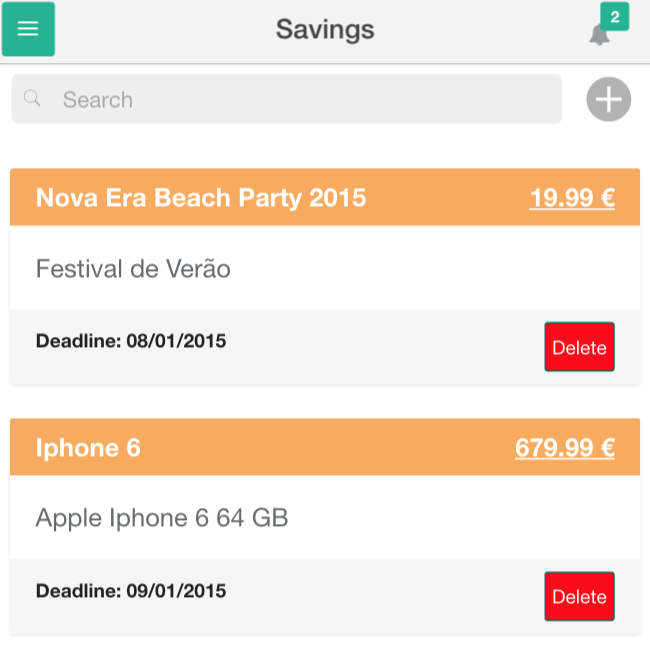
\includegraphics[width=0.5
		\textwidth]{savings/savings.png}
	\end{center}
	\caption{Poupanças Ativas}
	\label{fig:7}
\end{figure}

As poupanças são metas que o utilizador pretende alcançar e são constituídas por uma data limite, um montante e a descrição da poupança. A Figura \ref{fig:7} apresenta a lista de poupanças do utilizador.

\begin{figure}[H]
	\begin{center}
		\includegraphics[width=0.5
		\textwidth]{savings/addSavings.png}
	\end{center}
	\caption{Adicionar Poupança}
	\label{fig:7_1}
\end{figure}

Para adicionar uma nova poupança seleciona-se o botão de adicionar presente no ecrã de lista de poupanças. Surge um novo ecrã onde é necessário preencher todos os dados referentes à poupança.

  \section{Regras}
  \begin{figure}[H]
	\begin{center}
		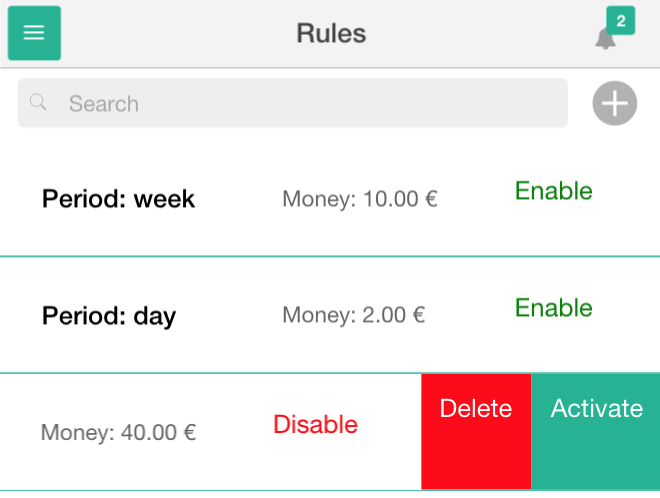
\includegraphics[width=0.5
		\textwidth]{rules/rules.png}
	\end{center}
	\caption{Regras Ativas e Desativas}
	\label{fig:8}
\end{figure}

As regras são constítuidas por periodo (dia, semana e mês), montante máximo que se pode gastar no periodo escolhido e o estado (ativa ou desativa). O objetivo é ajudar o utilizador a controlar os seus custos. Os pagamentos são autorizados apenas se cumprirem as regras e podem ser criadas pelo utilizador ou pelos pais com o objetivo de controlar os pagamentos dos filhos. As regras apenas podem ser eliminadas ou alteradas pelos pais ou pelos filhos caso estes a tenham criadas (ver Figura \ref{fig:8}).

\begin{figure}[H]
	\begin{center}
		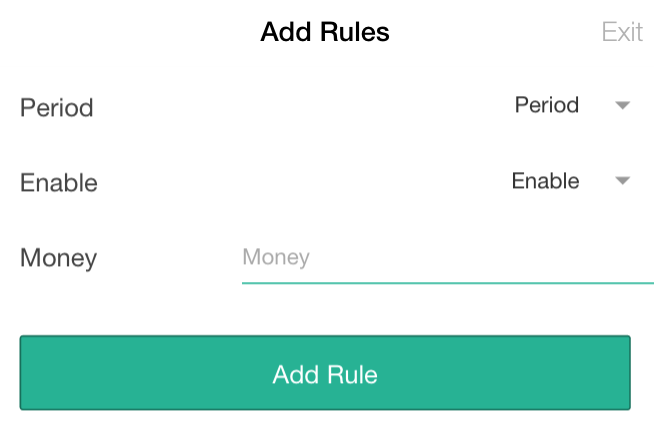
\includegraphics[width=0.5
		\textwidth]{rules/addRule.png}
	\end{center}
	\caption{Adicionar Regra}
	\label{fig:8_1}
\end{figure}

Para adicionar uma nova regra clica-se no botão de adcionar e preenche-se os dados do formulário apresentado na Figura \ref{fig:8_1}.  

  \section{Configurações}
  \label{sec:conf}
  \begin{figure}[H]
	\begin{center}
		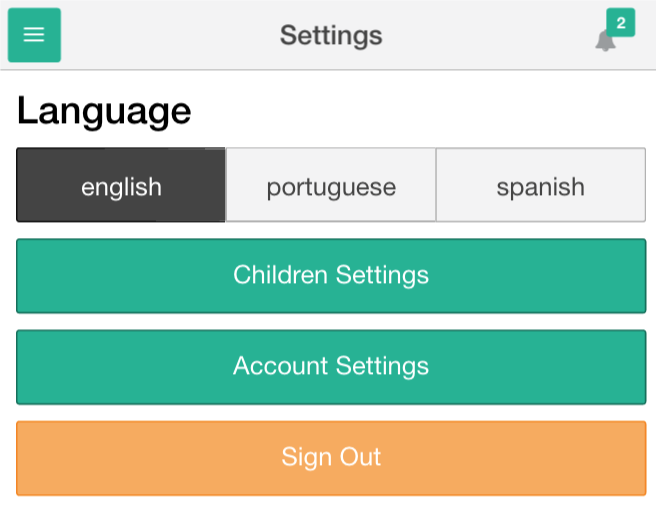
\includegraphics[width=0.5
		\textwidth]{settings/settings_menu.png}
	\end{center}
	\caption{Menu de Configurações}
	\label{fig:9}
\end{figure}

A Figura \ref{fig:9} apresenta as opções de configuração. É possível alterar o idioma, associar filhos à conta do utilizador e alterar informação da conta (ver Figura \ref{fig:9}).

\begin{figure}[H]
	\begin{center}
		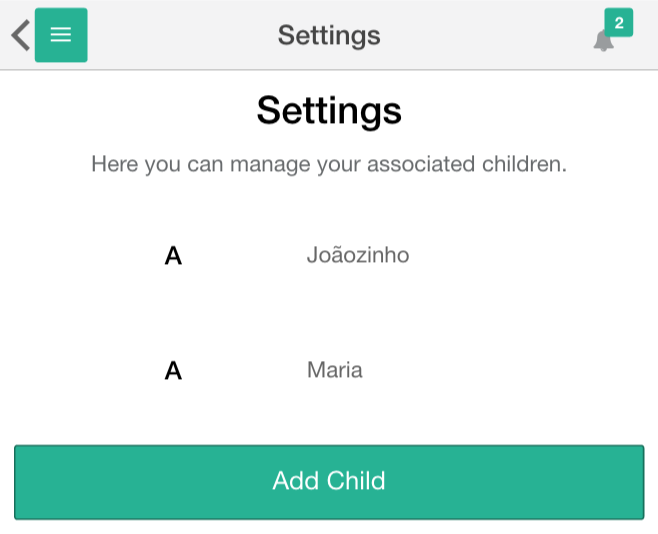
\includegraphics[width=0.5
		\textwidth]{settings/child_settings.png}
	\end{center}
	\caption{Adicionar Filho}
	\label{fig:9_1}
\end{figure}

Para associar um filho é necessário selecionar a opção definição dos filhos, de seguida a opção adicionar filho e por fim inserir o email e password para a conta do filho. Depois o filho pode autenticar-se e utilizar a aplicação.

\begin{figure}[H]
	\begin{center}
		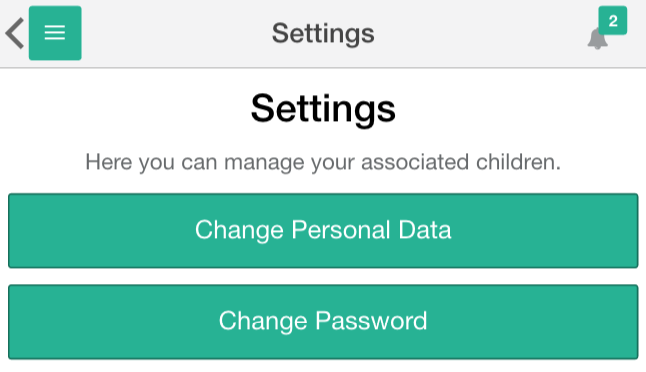
\includegraphics[width=0.5
		\textwidth]{settings/account_settings.png}
	\end{center}
	\caption{Configurar Conta}
	\label{fig:9_2}
\end{figure}

A Figura \ref{fig:9_2} apresenta as opções de alteração da informação da conta: alteração da informação e da \textit{password}. 

\begin{figure}[H]
	\begin{center}
		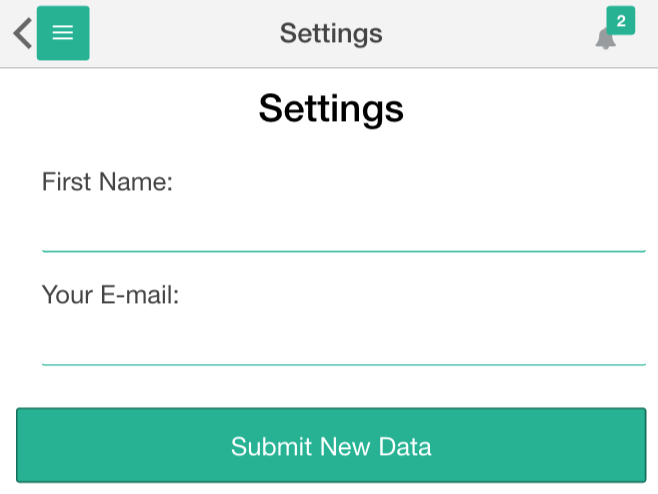
\includegraphics[width=0.5
		\textwidth]{settings/change_account.png}
	\end{center}
	\caption{Alterar Informação da Conta}
	\label{fig:9_3}
\end{figure}

\begin{figure}[H]
	\begin{center}
		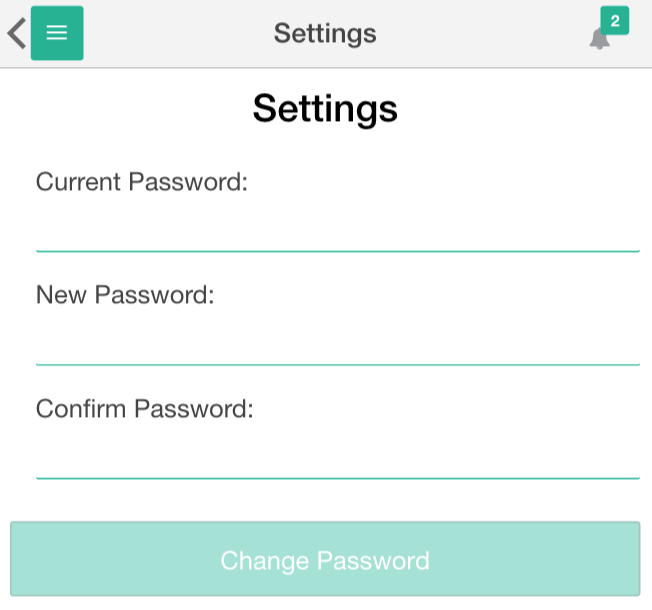
\includegraphics[width=0.5
		\textwidth]{settings/change_password.png}
	\end{center}
	\caption{Alterar \textit{Password}}
	\label{fig:9_4}
\end{figure}

As Figuras \ref{fig:9_3} e \ref{fig:9_4} apresentam, respetivamente, o ecrã de alteração de informação da conta e de alteração da \textit{password}.

\end{document}
